\section{Komplekse Tal}

Formålet med dette afsnit er at give en kort introduktion til komplekse tal, da det er et vigtigt redskab i store dele af fysikken. Vi vil her ikke gå i dybden med den stringente matematiske konstruktion af de komplekse tal, men i stedet fokusere på anvendelse og forskellige specifikke egenskaber, der er relevante for de ting, som vi skal arbejde med på campen.\\

Før vi definerer, hvad komplekse tal er, vil vi først kigge på den imaginære enhed $i$, som er meget vigtigt i forhold til at beskrive, hvad komplekse tal er. Den imaginære enhed er defineret som følger
%
\begin{align}
    i^2 = -1,
\end{align}
%
og blev oprindeligt indført som løsningen til ligningen $x^2 = -1$, der ikke kan løses med reelle tal. Men med den imaginære enhed kan man løse denne type ligning på følgende måde
%
\begin{align}
    x^2 = -1 \quad \Rightarrow \quad x^2 = i^2 \quad \Rightarrow \quad x = \pm \sqrt{i^2} = \pm i.
\end{align}
%
Det virker måske lidt underligt, sådan at indføre et nyt tal som $i$ for at løse en ligning, men det skal understreges at tallet $i$ er et tal ligesom som de reelle tal og at indførelsen af det ikke er anderledes matematisk set end indførelsen af negative tal. Nu hvor vi har indført den imaginære enhed, er vi nu klar til at give definitionen på et komplekst tal $z$. Definitionen lyder 
\begin{equation}
    z = a+ib,
\label{mat:eq:kompleks_def}
\end{equation}  
hvor $a$ og $b$ er reelle tal, der kaldes henholdsvis realdelen og imaginærdelen\footnote{At $b$ kaldes imaginærdelen skyldes, at tal på formen $ib$, hvor $b$ er et reelt tal, kaldes for imaginære tal.} af det komplekse tal $z$.  Dette skrives ofte som $\text{Re}(z) = a$ og $\text{Im}(z) = b$. En god måde at give en visuel beskrivelse af komplekse tal er vha. \emph{den komplekse plan}, som er illustreret i \cref{mat:fig:complex_plane}. Ligesom man normalt deler en plan op vha. en  $x$- og $y$-akse for at lave et koordinatsystem, deler man her den komplekse plan op vha. en real- og imaginærakse. Man kan således repræsentere ethvert komplekst tal, $z$, som et punkt i den komplekse plan, som det også er vist i \cref{mat:fig:complex_plane}. Denne visuelle repræsentation er god at have i baghovedet, da den viser at komplekse tal har to frihedsgrader, ligesom punkter i et koordinatsystem, $(x,y)$.
\begin{figure}[t]
	\centering
	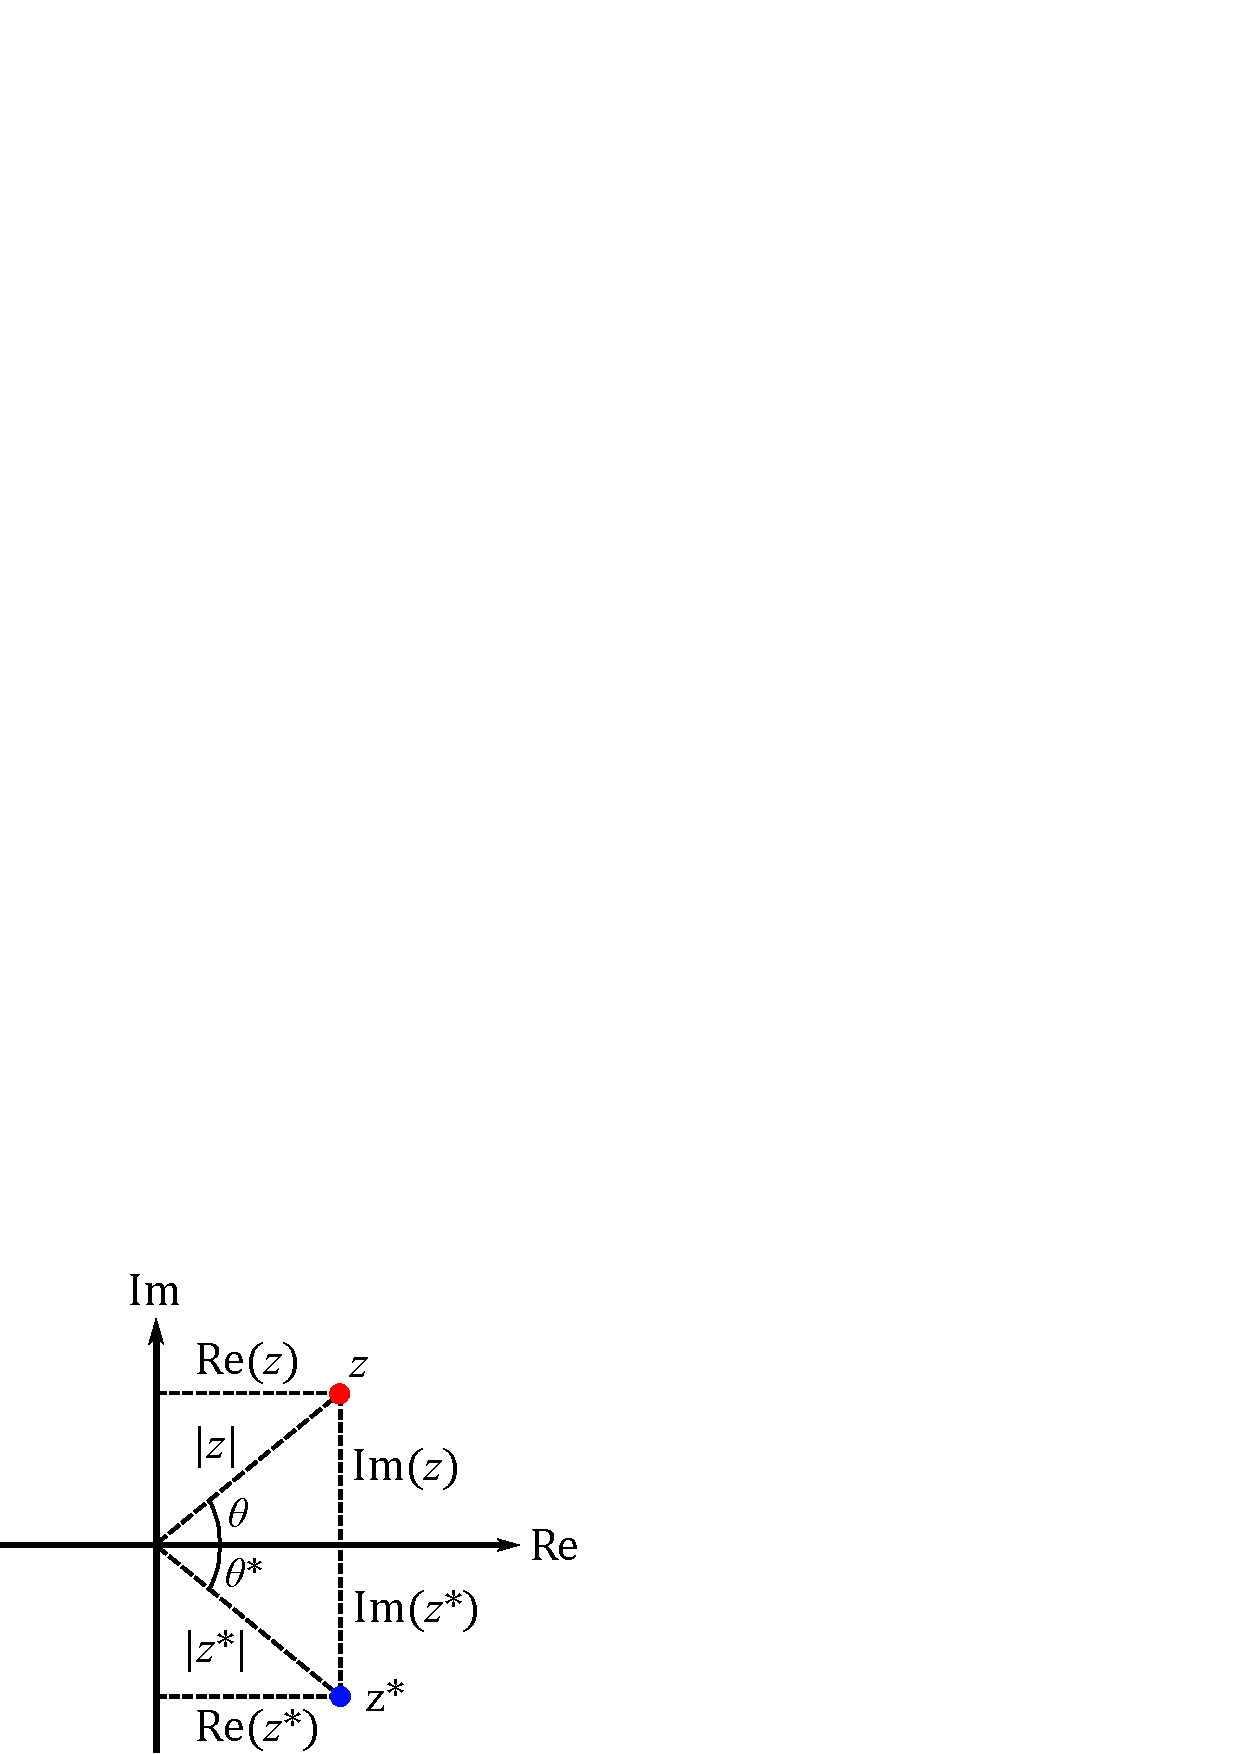
\includegraphics[width=0.5\textwidth]{Matematik/matfig/complex_plane.pdf}
	\caption{Et komplekst tal $z$ indikeret med en rød prik i det komplekse plan, samt dens kompleks konjugerede indikeret med en blå prik.}
	\label{mat:fig:complex_plane}
\end{figure} 

\noindent
Det næste spørgsmål vi skal kigge på er, hvordan man regner med komplekse tal. Mere specifikt skal vi starte med at kigge på \emph{addition, subtraktion, multiplikation} og \emph{division}, da disse regneoperationer lægger fundamentet for langt de fleste beregninger, som involverer komplekse tal. Lad derfor $z_1 = a+ib$ og $z_2 = c+id$ være to komplekse tal, og starte med at kigge på addition og subtraktion. Dette er defineret på den naturlige måde
\begin{subequations}
\begin{align}
    \label{mat:eq:kompleks_add}
    z_1+z_2 = (a+c) + i(b+d), \\
    \label{mat:eq:kompleks_sub}
    z_2-z_2 = (a-c) + i(b-d).
\end{align}
Man lægger/trækker altså realdelene og imaginærdelene til/fra hinanden hver for sig. Når man skal gange komplekse tal sammen, gøres det ganske som man ville forvente. Man regner blot som om, man gangede to parenteser ud
%
\begin{align*}
    z_1 z_2 = (a+bi)(c+id) = ac + iad + ibc + i^2bd = (ac-bd) + i(ad+bc),
\end{align*}
%
hvilket giver os definitionen for multiplikation af komplekse tal
\begin{equation}
    \label{mat:eq:kompleks_mul}
    z_1z_2 = (ac-bd) +i(ad+bc).
\end{equation}
Endeligt er der division, som kan defineres ud fra multiplikation. Dette kan illustreres ved følgende beregning
%
\begin{align*}
    \frac{z_1}{z_2} = \frac{a+ib}{c+id} = \frac{a+ib}{c+id} \cdot \frac{c-id}{c-id} = \frac{(ac+bd) + i(bc-ad)}{c^2 + d^2} = \frac{ac+bd}{c^2 + d^2} + i \frac{bc-ad}{c^2 + d^2},
\end{align*}
%
og definitionen for division af komplekse tal kan da skrives
\begin{equation}
    \label{mat:eq:kompleks_div}
    \frac{z_1}{z_2} = \frac{ac+bd}{c^2+d^2} + i\frac{bc-ad}{c^2+d^2}.
\end{equation}
\end{subequations}
Nu da de grundlæggende regneregler for komplekse tal er blevet gennemgået, vil vi gå videre og kigge på nogle af de andre vigtige definitioner og egenskaber ved de kompleks tal. Den første af disse er det, der kaldes for den \emph{komplekst konjugerede} af et komplekst tal $z$, og som skrives $z^*$. Hvis vi skriver $z = a+ib$ kan den komplekst konjugerede defineres som
\begin{equation}
    z^* = a - ib.
\end{equation}
Man finder således den komplekst konjugerede af et komplekst tal $z$ ved at skifte fortegn på imaginærdelen\footnote{Notationen $z^*$ for den komplekst konjugerede af et kompleks tal $z$ er meget almindelig i fysik. I matematik ses ofte notationen $\bar{z}$, men den bruges meget sjældent i fysik, hvor en streg ofte bruges til andre ting. Vi holder os derfor til notationen $z^*$.}. En kompleks konjugering kan derfor også ses, som en spejling af et komplekst tal i realaksen, se \cref{mat:fig:complex_plane}. Den næste egenskab ved komplekse tal er det, der kaldes for tallets \emph{modulus}, og som skrives $\abs{z}$. Definitionen af modulus er
\begin{equation}
    \abs{z} = \sqrt{a^2 + b^2},
\end{equation}
og kigger vi igen på \cref{mat:fig:complex_plane}, kan man vha. Pythagoras sætning se, at modulus for et komplekst tal angiver afstanden fra den komplekse plans origo (centrum) ud til det komplekse tal i planen. Ud fra definitionen af modulus kan man også vise følgende praktiske regneregler
\begin{subequations}
\begin{align}
    \abs{z} &= \abs{z^*}  \ , \label{mat:eq:modulus_regneregler1} \\
    \abs{z_1 z_2} &= \abs{z_1} \abs{z_2} \ , \label{mat:eq:modulus_regneregler2} \\
    \abs{z^n} &= \abs{z}^n \ . \label{mat:eq:modulus_regneregler3}
\end{align}
\end{subequations}
Dette bringer os videre til \emph{normkvadratet} for komplekse tal\footnote{Grunden til at det kaldes for et normkvadrat er, at modulus $|z|$ også i nogle sammenhænge kaldes for normen af $z$. Her holder vi os dog til at kalde $|z|$ for modulus og $|z|^2$ for normkvadratet.}, der er defineret som følger
\begin{equation}
    \label{mat:eq:normkvadrat}
    \abs{z}^2 = a^2 + b^2.
\end{equation}
Således er der som sådan ikke så meget nyt ved normkvadratet i forhold til modulus, men da normkvadratet ofte optræder i fysik, er det vigtigt at nævne alligevel. Specielt er følgende lighed god at kende
\begin{equation}
    \label{mat:eq:normkvadrat2}
    \abs{z}^2 = zz^*,
\end{equation} 
og kan nemt eftervises ved en hurtig beregning. Det sidste vi skal kigge på her er \emph{Eulers formel}, som er en af de mest brugbare relationer indenfor komplekse tal. Eulers formel siger at
\begin{equation}
    \label{mat:eq:Eulers_formel}
    e^{ix} = \cos(x) + i \sin(x),
\end{equation}
hvor $x$ er et reelt tal. Dette virker nok som en lidt underlig lighed, og det er umiddelbart også svært at se, hvad en eksponentialfunktion har med cosinus og sinus at gøre. Ikke desto mindre er formlen rigtig, og den er faktiske ikke så svær at bevise igen, hvorfor vi vender tilbage til det i \cref{mat:sec:raekker}. Tilgengæld vil vi påpege, at $e^{ix}$ har en pæn visuel repræsentation, som mængden af alle punkter på enhedscirklen (cirklen med radius 1 og centrum i origo) i den komplekse plan\footnote{Mængden af tal på formen $e^{ix}$ kaldes også for U(1) i gruppeteori, hvilket er særligt vigtigt i partikelfysik, hvor standardmodellen kan opsummeres som symmetrigruppen U(1)$_Y\times$SU(2)$_L\times$SU(3)$_C$, der dog har det problem, at intet kan have masse. Dette kan dog fikses med Higgsmekanismen, som Peter Higgs fik nobelprisen i 2013 for, hvilket reducerer stadardmodellen til symmetrigruppen U(1)$_Q\times$SU(3)$_C$. Det er dog en historie til en anden gang.}. I den visuelle repræsentation af de komplekse tal er modulus afstanden fra origo til det komplekse tal. Multipliceres Eulers formel med modulus fås
%
\begin{align} \label{mat:eq:pol_form_1}
    |z|e^{i\theta} = |z|\Big(\cos(\theta) + i \sin(\theta)\Big),
\end{align}
%
og sammenlignes dette med \cref{mat:eq:kartesisk/polaer} ses at realdelen har samme form som et $x$-koordinat, mens imaginærdelen har samme form som et $y$-koordinat. Ergo minder \cref{mat:eq:pol_form_1} om de polære koordinater fra \cref{mat:sec:trig}, hvorfor
%
\begin{align} \label{mat:eq:pol_form}
    z = |z|e^{i\theta}
\end{align}
%
også kaldes for et kompleks tals polære form. \\
En sidste vigtig ting, at nævne, er at man ofte bruger en anden notation for eksponentialfunktionen,
%
\begin{align}
    \exp(x) = e^x,
\end{align}
%
hvilket er smart, hvis der skal stå et langt udtryk på $x$' plads.